\documentclass[a4]{article}

\usepackage[icelandic]{babel}
\usepackage[T1]{fontenc}
\usepackage{amsmath}
\usepackage{graphicx}
\usepackage{sidecap}
\usepackage[utf8]{inputenc}
\usepackage[left=1in,top=1in,right=1in,bottom=1in,nohead]{geometry}
\usepackage[framed,numbered,autolinebreaks,useliterate]{../mcode}
\usepackage{amsfonts}
\usepackage{epstopdf}

\title{Töluleg Greining\\ Heimaverkefni 2}
\date{\today{}}
\author{ 
  Bjarki Geir Benediktsson,\and
  Haukur Óskar Þorgeirsson,\and
  Matthías Páll Gissurarson \and
  Kennari: Máni Maríus Viðarsson
  }



\begin{document}
\begin{flushright}
  Bjarki Geir Benediktsson,\\
  Haukur Óskar Þorgeirsson,\\
  Matthías Páll Gissurarson\\
\end{flushright}

\begin{center}
 \textsc{ \LARGE Töluleg Greining\\
  Heimaverkefni 2\\
  \today{}
  }
  \end{center}
\vfill

\maketitle
\section*{Inngangur}
%Bæta við texta
%%%%%%%%%%%%%%
%%%%%%%%%%%%%%
%%%%%%%%%%%%%%
%%%%%%%%%%%%%%
%%%%%%%%%%%%%%
%%%%%%%%%%%%%%
\section{Feristeikning með splæsibrúun}
\subsection{Teikning með aflestri af skjá}
\subsection{Teikning á lokuðum ferlum með aflestri af skjá}
\lstinputlisting{splaesiSkja_1.m}
%Bæta við mynd af keyrslu

\subsubsection{Teikning á þvinguðum ferlum með aflestri af skjá }
\lstinputlisting{splaesiSkja_2.m}
%Bæta við mynd af keyrslu
\subsection{Ferilteikning með Bezier-splæsibrúun}
\lstinputlisting{bezier_bruun3.m}
Fallið baz þjónar sama tilgangi fyrir Bezier brúunina og splaesi gerði fyrir splæsibrúunina það tekur við lista af fjórum hnitum $(x_i)_{i=0}^3$ og lista $(t_i)_{i=1}^n$ af gildum á $[0,1]$ og skilar lista af gildum $(r(t_i))_{i=1}^n$ þar sem  r 
$$r(t)=(1-t)^3x_0+3(1-t)^2tx_1+3(1-t)t^2x_2+t^3x_3$$
nú fæst að með því að gefa baz y-hnit í stað x-hnita sem inntak skilar það lista af $s(t)$ gildum þar sem  
$$s(t)=(1-t)^3y_0+3(1-t)^2ty_1+3(1-t)t^2y_2+t^3y_3$$
en það eru þau gildi sem við þurfum til að geta framkvæmt Bezier brúunina
\lstinputlisting{baz.m}
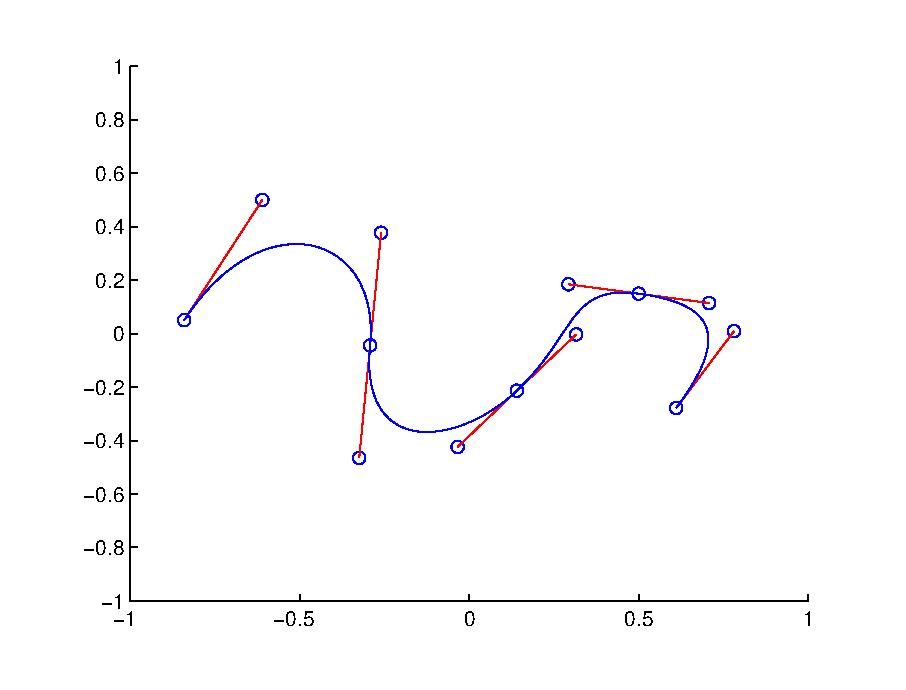
\includegraphics[height=0.495\textheight]{mynd21.eps}\\
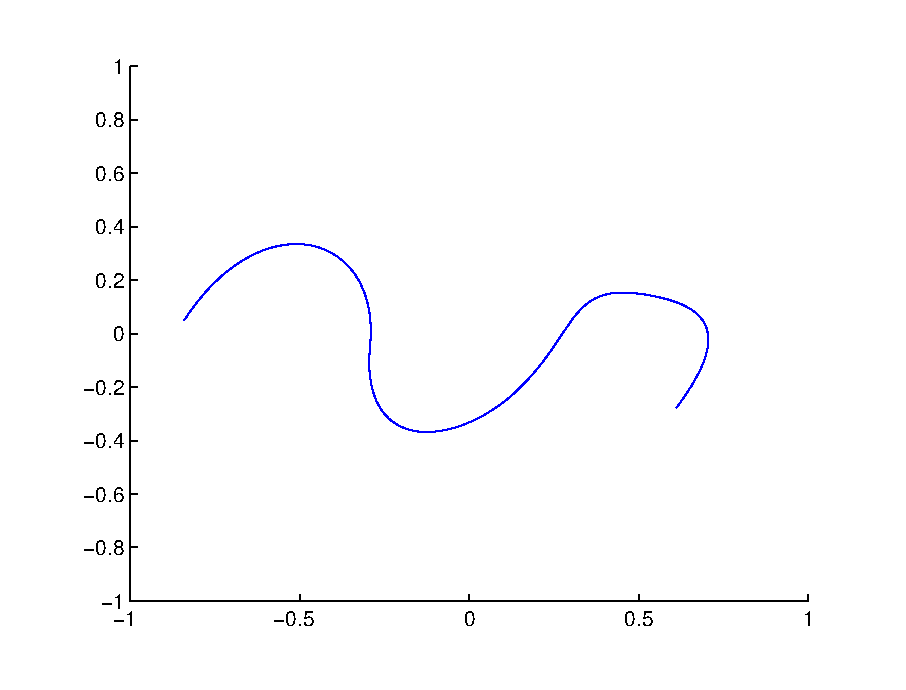
\includegraphics[height=0.495\textheight]{mynd22.eps}\\
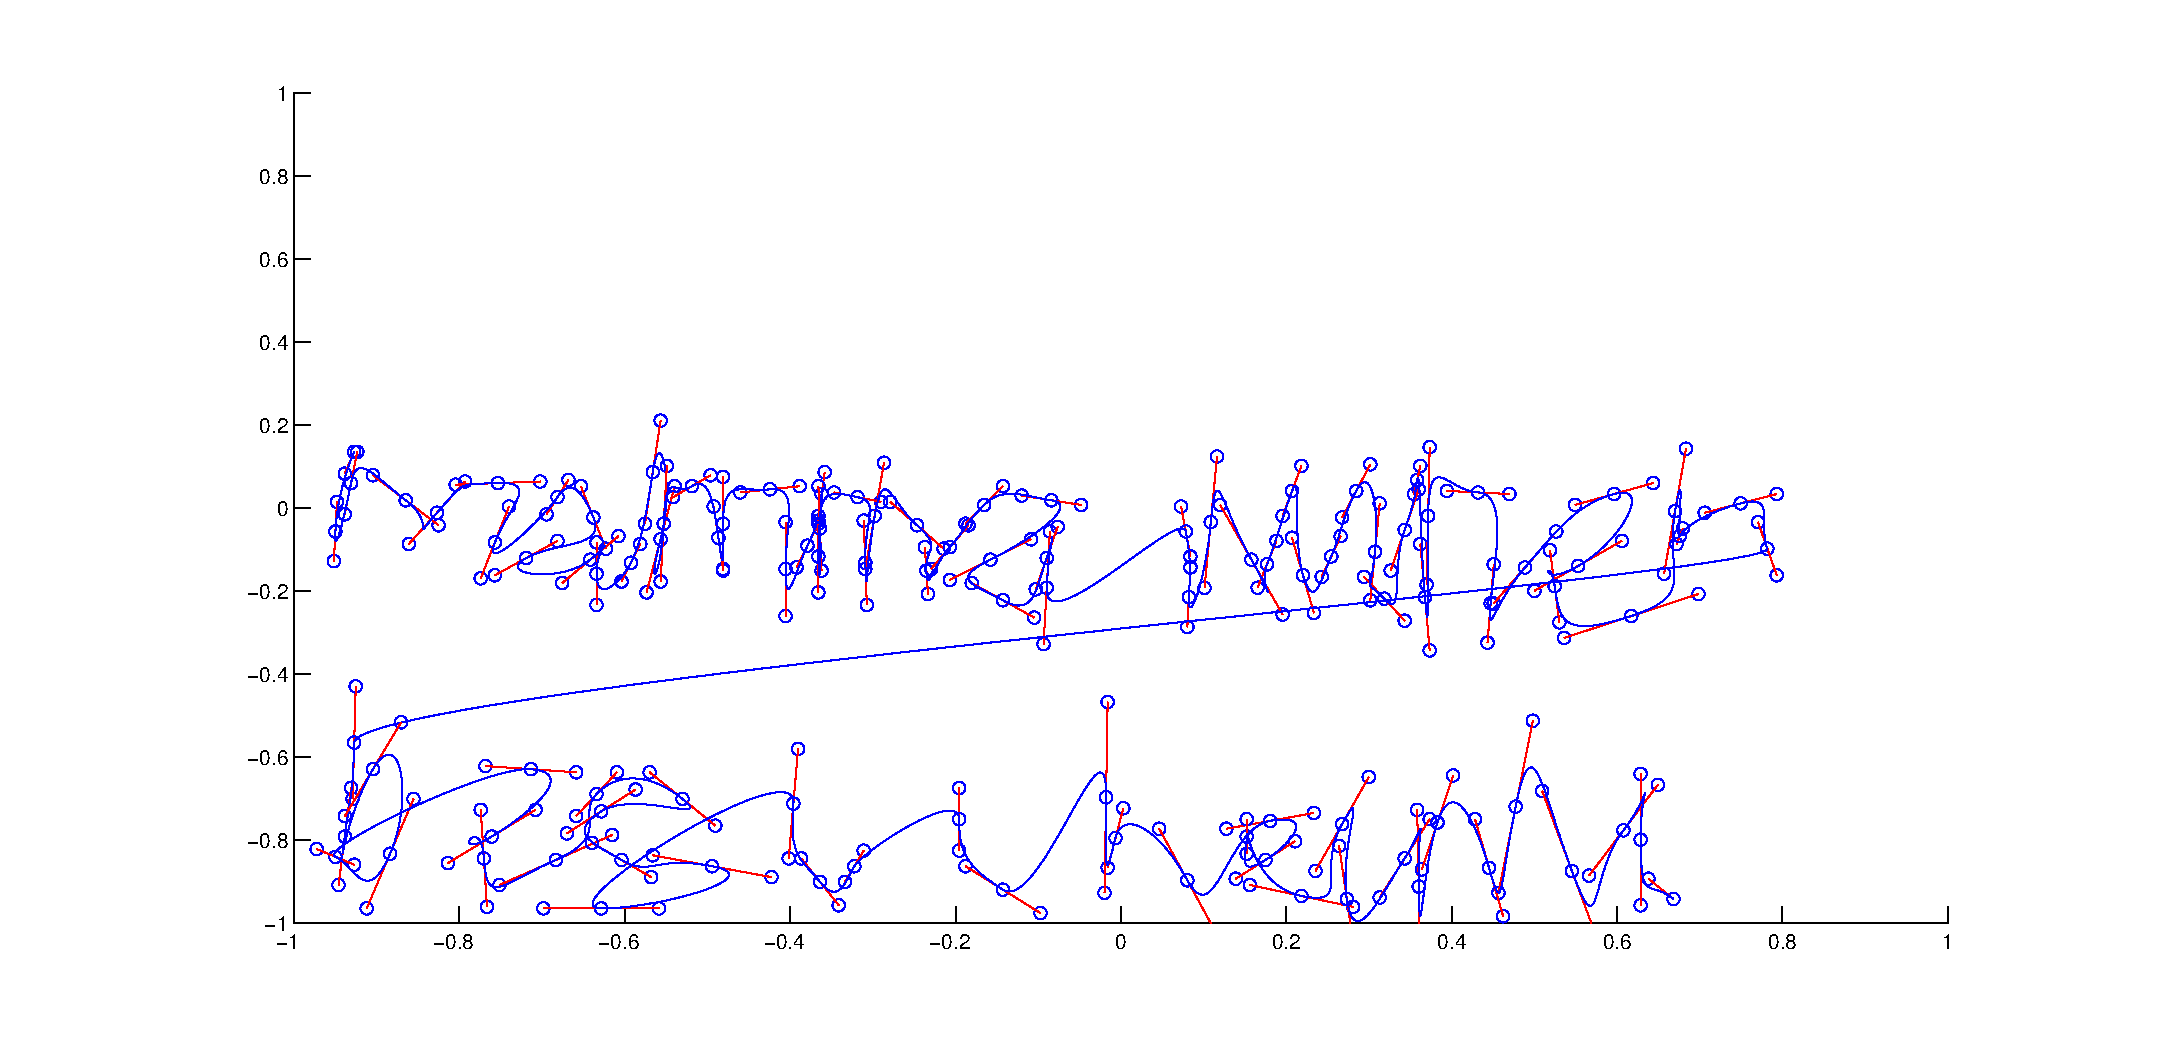
\includegraphics[width=\textwidth]{mamma1.eps}\\
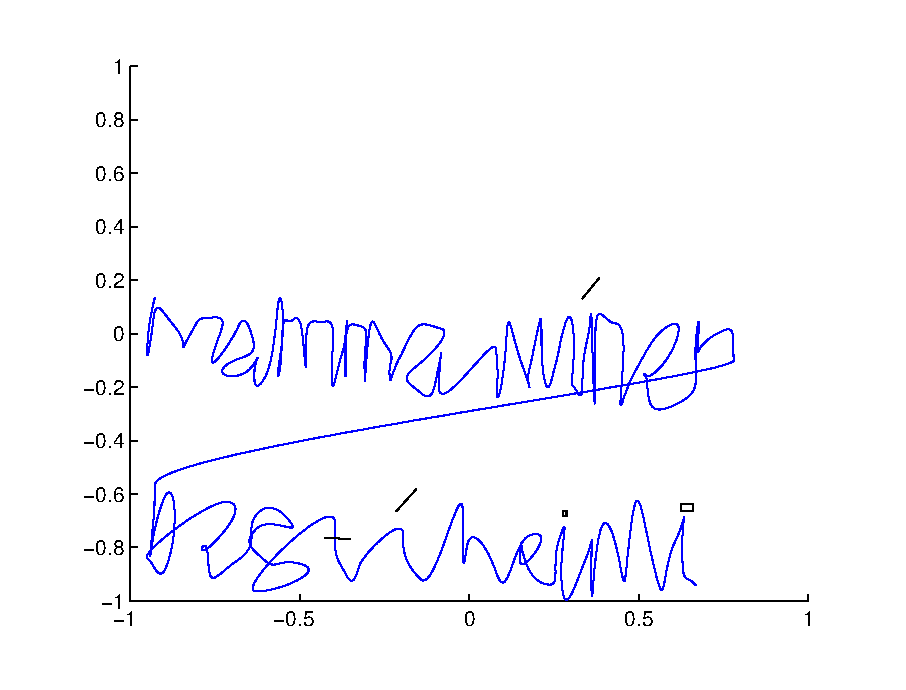
\includegraphics[height=0.495\textheight]{mamma2.eps}\\
hér mætti leyfa notenda að rjúfa ferilin með það er að vera með punkta sem ekki væri teiknað á milli 
Auk þess væri mjög sniðugt að geta hreyft punktana eftir að þeir hafa verið settir inn til að laga ferilin til
%Hér á að hafa inni fullt af myndarunki
\section{Nálgun á afleiðum,heildu, stiglum og Hessefylkjum}
\subsection{Almenn útgiskun}
\inputlstlisting{extrapolation.m}

\subsection{Richardson}
\subsection{Romberg}
\subsection{Nálgun á stiglum}
\subsection{Nálgun á Hessefylkjum}
\vspace{20 mm}
Að skýrsluni unnu :
\hspace{0.5cm} \makebox[1.5in]{\hrulefill}
\hspace{0.5cm} \makebox[1.5in]{\hrulefill}
\hspace{0.5cm} \makebox[1.5in]{\hrulefill}
\end{document}
